% !TeX root = spherical_harmonics.tex
% !TeX spellcheck = de_DE
\subsection{Die Suche nach einer guten Basis}
Auch wenn wir eingangs in unserem Kurs so sehr über Basen geschimpft haben\footnote{Wir wollen keine Namen nennen, aber Johannes war besonders hartnäckig...}, so ist uns natürlich bewusst, dass gerade für effiziente Berechnungen eine Basis praktisch immer gewählt wird. Welche Basis man wählt, ist dabei von großer Bedeutung: Andrea hat in ihrer Doktor-Arbeit eine bestimmte Berechnung, welche z.B. zur Modellierung von Luftbewegung millionenfach wiederholt genutzt werden soll, um den Faktor 1000 verschnellern können, und das nur durch geschickte Basiswahl. 

\begin{remark}
	Meistens ist eine Basis geschickt gewählt, wenn sie orthogonal bzgl. eines zum Problem passenden Skalarprodukts ist. Nun gibt es aber viele Skalarprodukte, die man wählen kann, die durchaus auch unterschiedliches Verständnis von Orthogonalität festlegen.
\end{remark}
Schauen wir uns einmal einige Beispiele für mögliche Skalarprodukte auf dem Raum der Polynome an:
\begin{example}
	Sei $B$ die Kugel in $\IR^3$ mit Radius 1. Dann ist mit
	\begin{align*}
		\braket{f,g}_B :&= \int_B f g \dd B
	\end{align*}
	ein Skalarprodukt auf dem Raum der Polynome gegeben.
\end{example}

\begin{example}
	Sei $Z$ ein Zylinder in $\IR^3$, z.B. mit Radius und Höhe 1. Dann ist mit
	\begin{align*}
		\braket{f,g}_Z :&= \int_Z f g \dd Z
	\end{align*}
	ein Skalarprodukt auf dem Raum der Polynome gegeben.
\end{example}

\begin{example}
	Sei $K$ ein Kegelstumpf in $\IR^3$, z.B. mit oberen Radius und Höhe 1 sowie unterem Radius $\frac{1}{2}$. Dann ist mit
	\begin{align*}
		\braket{f,g}_K :&= \int_K f g \dd K
	\end{align*}
	ein Skalarprodukt auf dem Raum der Polynome gegeben.
\end{example}

\begin{example}
	Sei $Q$ ein Quader in $\IR^3$, z.B. mit den Kantenlängen 1, 2 und 3. Dann ist mit
	\begin{align*}
		\braket{f,g}_Q :&= \int_Q f g \dd Q
	\end{align*}
	ein Skalarprodukt auf dem Raum der Polynome gegeben.
\end{example}

\begin{centralquestion}
Wäre es nicht praktisch, eine Basis zu finden, die für möglichst viele Skalarprodukte orthogonal ist? Wie würdet ihr mit dem neu erworbenen Wissen nach solch einer Basis suchen?

Diskutiert über eure Ansätze und versucht einen Algorithmus zu entwickeln, der eine möglichst allgemein einsetzbare Basis konstruiert.
\end{centralquestion}

\pagebreak
%\begin{remark}
%Am besten wählt man eine Basis, die möglichst gut an das gegebene Problem angepasst ist, doch was genau heißt das? Für die Auswahl an Problemen in diesem Kurs haben wir festgelegt, dass es sich um Probleme in unserer physikalischen Welt handeln soll. Wir haben uns bereits angeschaut, wie sich diese Einschränkung mathematisch äußert: Alles was wir messen wollen, muss natürlich, also $O_3$-verträglich sein. Wir haben uns auch schon mit der Darstellungstheorie von $O_3$ und einigen ihrer Untergruppen beschäftigt und festgestellt, dass $O_3$ den Raum der Polynome (oder äquivalent: den Raum der symmetrischen Tensoren) in irreduzible Unterräume zerlegt.
%\end{remark}
%\begin{remark}
%Die irreduziblen Unterräume sind besonders: Wir haben bereits sehr gut verstanden, dass sie immer (also für jedes $O_3$-verträgliche Skalarprodukt) senkrecht zueinander stehen und dass lineare Abbildungen zwischen zwei irreduziblen Unterräumen entweder 0 oder ein Vielfaches der Identität sein können. Wenn man also eine lineare Wirkung berechnen möchte, erspart man sich durch die Zerlegung in irreduzible Unterräume einiges an Arbeit: Alles, was zu bestimmen ist, sind die Konstanten, mit der die Identität zwischen zwei zueinander isomorphen irreduziblen Unterräumen koppeln.
%\end{remark}
%\begin{remark}
%Im übrigen: Für bilineare Abbildungen ist es etwas komplizierter, aber die grundsätzliche Aussage bleibt bestehen: Alle Abbildungen sind entweder 0 oder Vielfache einer Identität (auch dann wenn die Identität etwas komplizierter zu berechnen ist).
%\end{remark}
%\begin{remark}
% All dies legt nahe, dass eine Basiswahl, die an die irreduziblen Unterräume angepasst ist, praktisch immer eine gute Idee ist. Jetzt sind diese irreduziblen Unterräume aber allermeistens nicht ein-dimensional, wie sucht man sich nun eine möglichst kanonische Basis aus?
%\end{remark}
%\begin{remark}
%	\label{rem:einbettung_in_physik}
% Hinzu kommt, dass die irreduziblen Unterräume zwar für ganz $O_3$ irreduzibel sind, aber es gibt einige Probleme in der Physik, die eher einer Einbettung von $O_2$ in $O_3$ gleichen, z.B. (Teilchen-) Kollision an einer Wand, eine ausgezeichnete Richtung haben, z.B. die Bewegung von geladenen Teilchen durch einen Kondensator, oder rotierende Systeme beschreiben (Einbettung von $SO_2$ in $O_3$.
%\end{remark}
%
% \begin{remark}
% 	Idealerweise ist unsere Basis auch für solche Fälle ausgelegt. Es stellt sich heraus, dass beide Probleme gleichzeitig gelöst werden können.
% \end{remark}

% \begin{remark}
% 	Idealerweise ist unsere Basis auch für solche Fälle ausgelegt. Es stellt sich heraus, dass beide Probleme gleichzeitig gelöst werden können.
 %\end{remark}
 \subsection{Die Gelfand-Zetlin Basis}
 \begin{definition}[Konstruktion der $\Gae\jae\el\soft\fae\aaa\en\dae$-$\Zae\jae\tae\el\iii\en$-$\Bae\aaa\sae\iue$ (Gelfand\footnote{Israel Gelfand, $\I\sae\rae\aaa\iii\el\soft$ $\Em\ooo\iii\ssae\jae\jae\wae\iii\tschae$ $\Gae\jae\el\soft\fae\aaa\en\dae$ (1913--2009), sowjetischer Mathematiker}-Zetlin\footnote{Michael Zetlin, $\Em\iii\xa\aaa\iii\el$ $\El\soft\wae\ooo\wae\iii\tschae$ $\Zae\jae\tae\el\iii\en$ (1924--1966), russ. Mathematiker und Physiker; Der Name wird leider auf viele verschiedene Weisen transkribiert, u.A. eben Zetlin (meist im dt. Sprachraum), aber auch Tsetlin (engl. Sprachraum), Zeitlin, Tseitlin, Ceitlin}-Basis]
 	\label{def:konstruktion_gz_basis}
	Sei $G$ eine Gruppe mit halb-einfacher Darstellung auf einem Vektorraum $V$ und $U^i_0$ einer der irreduziblen Unterräume von $V$. Für diesen Unterraum wird eine \emph{Gelfand-Zetlin-Basis} wie folgt konstruiert:
	\begin{enumerate}[label={\arabic*.)}]
		\item Setze das Level $l=0, H_0 = G$
		\item Bestimme für jeden Unterraum $U_l^i$: \label{def:gz_it_anfang}
		\begin{enumerate}
			\item Berechne $\dim{U_l^i}$
			\item Ist $U_l^i$ 1-dimensional? Dann wähle einen von Null verschiedenen Vektor aus $U_l^i$ als einen der Basisvektoren von $U^1_0$.
			\item Ist $U_l^i$ mehr als $1$-dimensional? Dann merke dir $U_l^i$ für den nächsten Schritt.
		\end{enumerate}
		\item Wähle geschickt eine Untergruppe $H_{l+1}$ von $H_{l}$, sodass jeder Unterraum $U_l^i$ mit $\dim{U_l^i}>1$ in für $H_{l+1}$ irreduzible Unterräume  zerfällt. Dabei müssen alle Unterräume, die von einem gemeinsamen $U_l^i$ stammen, paarweise nicht isomorph sein (Klappt dies nicht, ist entweder eine andere Untergruppe zu finden, oder es gibt keine Gelfand-Zetlin-Basis). \label{def:gz_it_ugschritt}
		\item Nummeriere die Unterräume des nächst-höheren Levels: Nenne alle für $H_{l+1}$ irreduziblen Unterräume $U_{l+1}^{1}, \ldots, U_{l+1}^{k}$, inklusive der bereits für $H_l$ 1-dimensionalen Unterräume.
		\item Erhöhe das Level um 1: $l++$. \label{def:gz_it_ende}
		\item Wiederhole die Schritte \ref{def:gz_it_anfang} bis \ref{def:gz_it_ende}, bis alle Unterräume vom nächst-höheren Level 1-dimensional sind.
		\item $l_{\text{max}} = l$
		\end{enumerate}
\end{definition}
\begin{remark}
	Formal betrachtet, brauchen die 1-dimensionalen Untervektorräume nicht für Schritt \ref{def:gz_it_ugschritt} ausgeschlossen werden. Sie werden für jede Untergruppe 1-dimensional bleiben und sich nicht weiter ändern, entsprechend braucht man sie für die weiteren Schritte auch nicht zu berücksichtigen.
\end{remark}
\begin{definition}[$\Gae\jae\el\soft\fae\aaa\en\dae$-$\Zae\jae\tae\el\iii\en$-$\Dae\jae\rae\jae\wae\ooo$ (Gelfand-Zetlin-Baum)]
	Mit der Konstruktion nach \ref{def:konstruktion_gz_basis} bauen wir einen Baum mit $l_{\text{max}}+1$ Leveln. Der Stammknoten ist $U_0^i$, die Blätter sind alle gefundenen 1-dimensionale Unterräume. Die Knoten zwischen dem Stammknoten und den Blättern entsprechen den irreduziblen Unterräumen der jeweiligen Level, die Kanten verbinden einen irreduziblen Unterraum $U$ eines Levels mit allen irreduziblen Unterräumen des nächst-höheren Levels, die aus $U$ im Schritt \ref{def:gz_it_ugschritt} herauskommen. Eindimensionale Unterräume, die bereits in kleineren Leveln auftreten, werden hier als Knoten auf jedem höheren Level wiederholt bis zum maximalen Level.
	Diesen Baum nennen wir \emph{Gelfand-Zetlin-Baum}. Er kann z.B. wie folgt aussehen:
	\begin{align*}
		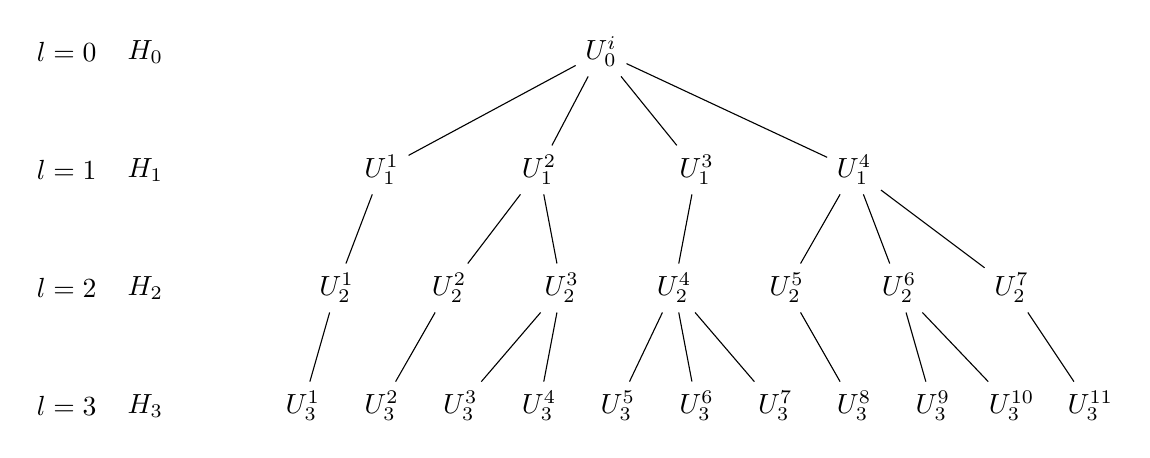
\begin{tikzpicture}[baseline={([yshift=-2ex]current bounding box.center)}]
			\foreach\x  in {1,2,...,11}{
				\node (u3\x) at (\x,-4.5){$U_3^{\x}$};
			}
%			\foreach\x  in {1,2,3.5,6,8,9.5,11}{
%				\node (u2\x) at (\x,-3){$U_2^{\x}$};
%			}
			\foreach\x [evaluate=\x as \y using {\x*10/7}] in {1,2,...,7}{
				\node (u2\x) at (\y,-3){$U_2^{\x}$};
			}
%			\foreach\x  in {1,2.75,6,9.5}{
%				\node (u1\x) at (\x,-1.5){$U_1^{\x}$};
%			}
			\foreach\x [evaluate=\x as \y using {\x*10/5}] in {1,2,...,4}{
				\node (u1\x) at (\y,-1.5){$U_1^{\x}$};
			}
			\node (u0) at (4.7875,0){$U_0^i$};
			\foreach\x in {1,2,...,4}{
				\draw[] (u0) to (u1\x);
			}
			\draw[] (u11) to (u21);
			\draw[] (u12) to (u22);
			\draw[] (u12) to (u23);
			\draw[] (u13) to (u24);
			\draw[] (u14) to (u25);
			\draw[] (u14) to (u26);
			\draw[] (u14) to (u27);
			\draw[] (u21) to (u31);
			\draw[] (u22) to (u32);
			\draw[] (u23) to (u33);
			\draw[] (u23) to (u34);
			\draw[] (u24) to (u35);
			\draw[] (u24) to (u36);
			\draw[] (u24) to (u37);
			\draw[] (u25) to (u38);
			\draw[] (u26) to (u39);
			\draw[] (u26) to (u310);
			\draw[] (u27) to (u311);
			\foreach\x [evaluate=\x as \y using {-\x*1.5}] in {0,1,...,3}{
				\node (l\x) at (-2,\y){$l=\x$};
				\node (h\x) at (-1,\y){$H_{\x}$};
			}
		\end{tikzpicture}
	\end{align*}
	In einem Gelfand-Zetlin-Baum sind alle Darstellungen paarweise ungleich. Es kann aber auftreten, dass manche Darstellungen isomorph zueinander sind (wobei die Kinder eines Knotens niemals isomorph zueinander sein dürfen).
\end{definition}
\begin{remark}
		Die Wahl der Untergruppen-Kette $H_1,\ldots,H_{l_{\text{max}}}$ ist hier spielentscheidend und keinesfalls eindeutig. Aus diesem Grund gehört zu einer vollständigen Anweisung \enquote{Wähle eine Gelfand-Zetlin-Basis für $G$ auf $V$} auch die Angabe der Untergruppenkette $H_1,\ldots,H_{l_{\text{max}}}$.
\end{remark}
\begin{remark}
	Auch wenn die Konstruktion einer Gelfand-Zetlin-Basis klappt, hat man nicht unbedingt etwas gewonnen. Wenn man dazu besonders exotische Untergruppen benutzen muss, bringt einem die Gelfand-Zetlin-Basis in der Anwendung nicht besonders viel. Eigentlich möchte man sich erst für eine Untergruppenkette $H_0,\ldots,H_{l_{\text{max}}}$ entscheiden und dann schauen, ob die Konstruktion funktioniert.
\end{remark}
\begin{definition}[$\Gae\jae\el\soft\fae\aaa\en\dae$-$\Zae\jae\tae\el\iii\en$-$\Bae\aaa\sae\aaa$]
	\label{def:gz_basis}
	Sei $G$ eine Gruppe mit Darstellung auf einem Vektorraum $V$ und $G$ zerlege $V$ in seine irreduziblen Unterräume $U^1_0,\ldots,U^k_0$. Wähle außerdem eine Untergruppenkette $H_1 \gneq\ldots\gneq H_{l_{\text{max}}}$. Für jeden dieser Unterräume wird nun einzeln eine Basis $\mathcal{B}$ konstruiert nach \ref{def:konstruktion_gz_basis}. $\mathcal{B}$ heißt dann \emph{Gelfand-Zetlin-Basis von der Darstellung V bezüglich} $H_1,\cdots H_{l_{\text{max}}}$. 
\end{definition}

\begin{remark}
	Wir sind insbesondere an der Darstellung von $O_3$ auf dem Polynomraum und der Einbettung von $O_2$, $SO_2$ bzw. $O_1$ interessiert. Praktischerweise gilt $O_3\gneq O_2\gneq SO_2$ und  $O_3\gneq O_2\gneq O_1$ und somit bilden die Gruppen $O_3, O_2, SO_2, O_1$ zwei Untergruppenketten.
\end{remark}

\begin{centralquestion}[Fortsetzung]\label{cq:fortsetzung}
	Kann man mit den beiden Untergruppenketten $O_3\gneq O_2\gneq SO_2$ und  $O_3\gneq O_2\gneq O_1$ dargestellt auf dem komplexen oder reellen Polynomraum eine Gelfand-Zetlin-Basis basteln? Wie sehen solche von uns gewünschte Basen nun konkret aus?

	Teilt euch in Gruppen auf und erstellt Gelfand-Zetlin-Bäume zu den vier Kombinationen
	\begin{align*}
		O_3\gneq O_2\gneq SO_2 \text{ dargestellt auf }& \IC[x,y,z] & O_3\gneq O_2\gneq SO_2 \text{ dargestellt auf }& \IR[x,y,z] \\
		O_3\gneq O_2\gneq O_1 \text{ dargestellt auf }& \IC[x,y,z] & O_3\gneq O_2\gneq O_1 \text{ dargestellt auf }& \IR[x,y,z]
	\end{align*}
	Hinweis: Eine der vier Fälle funktioniert nicht -- warum?
\end{centralquestion}

\pagebreak
\begin{maintheorem}[Spherical Harmonics sind eine Gelfand-Zetlin-Basis]\label{mt:sh_sind_gzb}
	Die Darstellung von $O_3$ auf dem Polynomraum (egal, ob mit reellen oder komplexen Koeffizienten) hat die Gelfand-Zetlin-Basis bezüglich Untergruppenkette $O_3 \geq O_2 \geq O_1$. Die Element dieser Basis heißen \emph{reelle Spherical Harmonics} oder auch \emph{Kugelflächenfunktionen}.

	Sofern man mit komplexen Koeffizienten arbeitet, gibt es eine zweite Gelfand-Zetlin-Basis bezüglich der Untergruppenkette $O_3 \geq O_2 \geq SO_2$. Die Elemente dieser Gelfand-Zetlin-Basis heißen \emph{komplexe Spherical Harmonics}.
\end{maintheorem}

\begin{lemma}[{Gelfand-Zetlin-Baum für $O_3\gneq O_2\gneq SO_2 \text{ dargestellt auf } \IC[x,y,z]$}]
	\begin{align*}
		\begin{tikzpicture}[baseline={([yshift=-2ex]current bounding box.center)}]
			\node (u20) at (0,-3){$\mathscr{E}_\IC^{0}$};
			\foreach\x [evaluate=\x as \y using {(\x)*2.5-0.5},evaluate=\x as \z using {(\x)*2.5+0.5}] in {1,2,3}{
				\node (u2m\x) at (\y,-3){$\mathscr{E}_\IC^{-\x}$};
				\node (u2p\x) at (\z,-3){$\mathscr{E}_\IC^{\x}$};
			}
			\node (u2m4) at (4*2.5-0.5,-3){$\cdots$};
			\node (u2p4) at (4*2.5+0.5,-3){$\cdots$};
			\node (u2m5) at (5*2.5-0.5,-3){$\mathscr{E}_\IC^{-k}$};
			\node (u2p5) at (5*2.5+0.5,-3){$\mathscr{E}_\IC^{k}$};
			\node (u10) at (0*10/5,-1.5){$^2\mathscr{H}_\IC^0$};
			\foreach\x [evaluate=\x as \y using {\x*2.5}] in {1,2,3}{
				\node (u1\x) at (\y,-1.5){$^2\mathscr{H}_\IC^{\x}$};
			}
			\node (u14) at (4*2.5,-1.5){$\cdots$};
			\node (u15) at (5*2.5,-1.5){$^2\mathscr{H}_\IC^k$};
			\node (u0) at (4.7875,0){$^3\mathscr{H}_\IC^k$};
			\foreach\x in {0,1,...,5}{
				\draw[] (u0) to (u1\x);
			}
			\foreach\x in {1,2,3,4,5}{
				\draw[] (u1\x) to (u2m\x);
				\draw[] (u1\x) to (u2p\x);
			}
			\draw[] (u10) to (u20);
			\foreach\x [evaluate=\x as \y using {-\x*1.5}] in {0,1,...,2}{
				\node (l\x) at (-2,\y){$l=\x$};
			}
			\node (h0) at (-1,0){$O_3$};
			\node (h1) at (-1,-1.5){$O_2$};
			\node (h2) at (-1,-3){$SO_2$};
		\end{tikzpicture}
	\end{align*}
\end{lemma}

\begin{lemma}[{Gelfand-Zetlin-Baum für $O_3\gneq O_2\gneq O_1 \text{ dargestellt auf } \IC[x,y,z]$}]
	\begin{align*}
		\begin{tikzpicture}[baseline={([yshift=-2ex]current bounding box.center)}]
			\node (u20) at (0,-3){$^1\mathscr{H}_\IC^{0}$};
			\foreach\x [evaluate=\x as \y using {(\x)*2.5-0.5},evaluate=\x as \z using {(\x)*2.5+0.5}] in {1,2,3,5}{
				\node (u2m\x) at (\y,-3){$^1\mathscr{H}_\IC^{0}$};
				\node (u2p\x) at (\z,-3){$^1\mathscr{H}_\IC^{1}$};
			}
			\node (u2m4) at (4*2.5-0.5,-3){$\cdots$};
			\node (u2p4) at (4*2.5+0.5,-3){$\cdots$};
			\node (u10) at (0*10/5,-1.5){$^2\mathscr{H}_\IC^0$};
			\foreach\x [evaluate=\x as \y using {\x*2.5}] in {1,2,3}{
				\node (u1\x) at (\y,-1.5){$^2\mathscr{H}_\IC^{\x}$};
			}
			\node (u14) at (4*2.5,-1.5){$\cdots$};
			\node (u15) at (5*2.5,-1.5){$^2\mathscr{H}_\IC^k$};
			\node (u0) at (4.7875,0){$^3\mathscr{H}_\IC^k$};
			\foreach\x in {0,1,...,5}{
				\draw[] (u0) to (u1\x);
			}
			\foreach\x in {1,2,3,4,5}{
				\draw[] (u1\x) to (u2m\x);
				\draw[] (u1\x) to (u2p\x);
			}
			\draw[] (u10) to (u20);
			\foreach\x [evaluate=\x as \y using {-\x*1.5}] in {0,1,...,2}{
				\node (l\x) at (-2,\y){$l=\x$};
			}
			\node (h0) at (-1,0){$O_3$};
			\node (h1) at (-1,-1.5){$O_2$};
			\node (h2) at (-1,-3){$O_1$};
		\end{tikzpicture}
	\end{align*}
\end{lemma}
\begin{lemma}[{Gelfand-Zetlin-Baum für $O_3\gneq O_2\gneq O_1 \text{ dargestellt auf } \IR[x,y,z]$}]
	\begin{align*}
		\begin{tikzpicture}[baseline={([yshift=-2ex]current bounding box.center)}]
			\node (u20) at (0,-3){$^1\mathscr{H}_\IR^{0}$};
			\foreach\x [evaluate=\x as \y using {(\x)*2.5-0.5},evaluate=\x as \z using {(\x)*2.5+0.5}] in {1,2,3,5}{
				\node (u2m\x) at (\y,-3){$^1\mathscr{H}_\IR^{0}$};
				\node (u2p\x) at (\z,-3){$^1\mathscr{H}_\IR^{1}$};
			}
			\node (u2m4) at (4*2.5-0.5,-3){$\cdots$};
			\node (u2p4) at (4*2.5+0.5,-3){$\cdots$};
			\node (u10) at (0*10/5,-1.5){$^2\mathscr{H}_\IR^0$};
			\foreach\x [evaluate=\x as \y using {\x*2.5}] in {1,2,3}{
				\node (u1\x) at (\y,-1.5){$^2\mathscr{H}_\IR^{\x}$};
			}
			\node (u14) at (4*2.5,-1.5){$\cdots$};
			\node (u15) at (5*2.5,-1.5){$^2\mathscr{H}_\IR^k$};
			\node (u0) at (4.7875,0){$^3\mathscr{H}_\IR^k$};
			\foreach\x in {0,1,...,5}{
				\draw[] (u0) to (u1\x);
			}
			\foreach\x in {1,2,3,4,5}{
				\draw[] (u1\x) to (u2m\x);
				\draw[] (u1\x) to (u2p\x);
			}
			\draw[] (u10) to (u20);
			\foreach\x [evaluate=\x as \y using {-\x*1.5}] in {0,1,...,2}{
				\node (l\x) at (-2,\y){$l=\x$};
			}
			\node (h0) at (-1,0){$O_3$};
			\node (h1) at (-1,-1.5){$O_2$};
			\node (h2) at (-1,-3){$O_1$};
		\end{tikzpicture}
	\end{align*}
\end{lemma}

\begin{lemma}[{Versuchter Gelfand-Zetlin-Baum für $O_3\gneq O_2\gneq SO_2 \text{ dargestellt auf } \IR[x,y,z]$}]
	\begin{align*}
		\begin{tikzpicture}[baseline={([yshift=-2ex]current bounding box.center)}]
			\node (u24) at (4*2.5,-3){$\cdots$};
			\foreach\x [evaluate=\x as \y using {\x*2.5}] in {0,1,2,3}{
				\node (u2\x) at (\y,-3){$^2\mathscr{H}_\IR^{\x}$};
				\node (u1\x) at (\y,-1.5){$^2\mathscr{H}_\IR^{\x}$};
			}
			\node (u14) at (4*2.5,-1.5){$\cdots$};
			\node (u25) at (5*2.5,-3){$^2\mathscr{H}_\IR^k$};
			\node (u15) at (5*2.5,-1.5){$^2\mathscr{H}_\IR^k$};
			\node (u0) at (4.7875,0){$^3\mathscr{H}_\IR^k$};
			\foreach\x in {0,1,...,5}{
				\draw[] (u0) to (u1\x);
			}
			\foreach\x in {0,1,2,3,4,5}{
				\draw[] (u1\x) to (u2\x);
			}
			\foreach\x [evaluate=\x as \y using {-\x*1.5}] in {0,1,...,2}{
				\node (l\x) at (-2,\y){$l=\x$};
			}
			\node (h0) at (-1,0){$O_3$};
			\node (h1) at (-1,-1.5){$O_2$};
			\node (h2) at (-1,-3){$SO_2$};
		\end{tikzpicture}
	\end{align*}
\end{lemma}

\begin{proof}
	Siehe vorherige Kapitel, insbesondere zur Darstellungstheorie von $O_3$.
\end{proof}

\begin{remark}
	Meistens werden einem Spherical Harmonics als Basis-Satz mit besonderen Eigenschaften vorgesetzt und nicht als Gelfand-Zetlin-Basis definiert. Es fehlt also noch die Überprüfung, dass die üblichen Spherical Harmonics auch mit der Definition nach \ref{mt:sh_sind_gzb} übereinstimmen.
\end{remark}
\begin{lemma}[Die Bezeichnung \enquote{Spherical Harmonics} ist gerechtfertigt]
	Die Gelfand-Zetlin-Basis von $O_3\gneq O_2\gneq SO_2 \text{ dargestellt auf } \IC[x,y,z]$ stimmt bis auf skalare Vielfache mit den komplexen Spherical Harmonics, wie sie üblicherweise gegeben sind, überein. Gleiches gilt für die Gelfand-Zetlin-Basis von $O_3\gneq O_2\gneq O_1 \text{ dargestellt auf } \IR[x,y,z]$ für die reellen Spherical Harmonics.

	Hierbei gilt zu beachten: Die Einbettung der Untergruppen in $O_3$ legt drei ausgezeichnete Raumrichtungen in Form von Fixpunkträumen fest: Die Drehachse $z$ ($O_2$ eingebettet in $O_3$),
\end{lemma}

\begin{definition}[Wikipedias Herleitung der Spherical Harmonics]
Die \emph{Kugelflächenfunktionen} sind ein vollständiger und orthonormaler Satz von Eigenfunktionen des Winkelanteils des Laplace-Operators. Dieser Winkelanteil zeigt sich, wenn der Laplace-Operator in Kugelkoordinaten geschrieben wird. Die Eigenwertgleichung lautet:

\[\left(\frac{\partial^{2}}{\partial\vartheta^{2}}+\frac{\cos\vartheta}{\sin\vartheta}\frac{\partial}{\partial\vartheta}+\frac{1}{\sin^{2}\vartheta}\frac{\partial^{2}}{\partial\varphi^{2}}\right)Y_{lm}(\vartheta,\varphi)=-l(l+1)Y_{lm}(\vartheta,\varphi)\]

Die Eigenfunktionen sind die Kugelflächenfunktionen $Y_{lm}(\vartheta,\varphi)$, dabei sind $N_{lm}$ Normierungsfaktoren und $P_{lm}(z)$ die zugeordneten Legendrepolynome (Details siehe unten):

\[Y_{lm}:\;\left[0,\pi\right]\times\left[0,2\pi\right]\rightarrow\mathbb{C},\quad(\vartheta,\varphi)\mapsto\frac{1}{\sqrt{2\pi}}\, N_{lm}\, P_{lm}(\cos\vartheta)\, e^{\mathrm im\varphi}\\
\quad \text{mit}\quad N_{lm} := \sqrt{\tfrac{2l+1}{2}\,\tfrac{(l-m)!}{(l+m)!}}\]

Besonders in der theoretischen Physik haben die Kugelflächenfunktionen eine große Bedeutung für die Lösung partieller Differentialgleichungen. Sie treten zum Beispiel bei der Berechnung von Atomorbitalen auf, da die beschreibende zeitunabhängige Schrödingergleichung den Laplace-Operator enthält und sich das Problem am besten in Kugelkoordinaten lösen lässt. Auch die in der Elektrostatik auftretenden Randwertprobleme können elegant durch die Entwicklung nach Kugelflächenfunktionen gelöst werden. In der Geophysik und Geodäsie werden die Kugelflächenfunktionen bei der Approximation des Geoids  und des Magnetfeldes verwendet.

\begin{description}
	\item[Zusammenhang mit dem Laplace-Operator]

Der Winkelanteil des Laplace-Operators zeigt sich, wenn dieser in Kugelkoordinaten geschrieben wird:

\[\Delta=\frac{\partial^{2}}{\partial r^{2}}+\frac{2}{r}\frac{\partial}{\partial r}+\frac{1}{r^{2}}\left(\frac{\partial^{2}}{\partial\vartheta^{2}}+\frac{\cos\vartheta}{\sin\vartheta}\frac{\partial}{\partial\vartheta}+\frac{1}{\sin^{2}\vartheta}\frac{\partial^{2}}{\partial\varphi^{2}}\right)=\Delta_{r}+\frac{1}{r^{2}}\Delta_{\vartheta,\varphi}\]

Der rechte, eingeklammerte Teil wird hier als \enquote{Winkelanteil} $\Delta_{\vartheta,\varphi}$ bezeichnet. Er ist direkt proportional zum Quadrat des Drehimpulsoperators $\hat{\mathbf{L}}^2=-\hbar^{2} \Delta_{\vartheta,\varphi}$.

Die Laplacesche Differentialgleichung in Kugelkoordinaten
\[
\Delta f(r,\vartheta,\varphi)\ = 0
\]
hat neben der trivialen Lösung, $f=0$, verschiedenste Lösungen mit vielen technischen Anwendungen.

Zur Lösung wird folgender Produktansatz verwendet, wobei $R_{l}(r)$ nur vom Radius und $Y_{lm}(\vartheta,\varphi)$ nur von Polar- und Azimutwinkel abhängt:
\[f(r,\vartheta,\varphi) = R_{l}(r) Y_{lm}(\vartheta,\varphi) \]

Dies ergibt eingesetzt:
\[\Delta R_{l}(r)Y_{lm}(\vartheta,\varphi)=Y_{lm}(\vartheta,\varphi)\Delta_{r}R_{l}(r)+\frac{R_{l}(r)}{r^{2}}\Delta_{\vartheta,\varphi}Y_{lm}(\vartheta,\varphi)=0\]

Multiplikation von $r^2$ und Division durch $R_{l}(r) Y_{lm}(\vartheta,\varphi)$ liefert:
\[\frac{r^{2}\Delta_{r}R_{l}(r)}{R_{l}(r)}+\frac{\Delta_{\vartheta,\varphi}Y_{lm}(\vartheta,\varphi)}{Y_{lm}(\vartheta,\varphi)}=0\]

Diese Gleichung kann nur erfüllt werden, wenn in beiden Summanden unabhängig voneinander Radius und Winkel variierbar sind. Beide Summanden müssen somit denselben konstanten Wert annehmen, der zu $l(l+1)$ gewählt wird (diese Festlegung erweist sich später als sinnvoll):
\[\frac{r^{2}\Delta_{r}R_{l}(r)}{R_{l}(r)}=l(l+1)=-\frac{\Delta_{\vartheta,\varphi}Y_{lm}(\vartheta,\varphi)}{Y_{lm}(\vartheta,\varphi)}\]

Durch dieses Verfahren, welches Separationsansatz genannt wird, wurde also das ursprüngliche Problem, nämlich die Lösung der Laplace-Gleichung (partielle Differentialgleichung mit drei unabhängigen Variablen), auf das einfachere Problem der Lösung einer gewöhnlichen Differentialgleichung (Radialgleichung)
\[\Delta_{r}R_{l}(r)=\frac{l(l+1)}{r^{2}}R_{l}(r)\]

und einer partiellen Differentialgleichung mit zwei unabhängigen Variablen (winkelabhängige Gleichung), die gerade von den Kugelflächenfunktionen erfüllt wird, reduziert.
\[\Delta_{\vartheta,\varphi}Y_{lm}(\vartheta,\varphi)=-l(l+1)Y_{lm}(\vartheta,\varphi)\]

Nun lässt sich aufgrund der Orthogonalität und Vollständigkeit der Kugelflächenfunktionen zeigen, dass sich jede quadratintegrable Funktion aus diesen speziellen Funktionen als Summe zusammensetzen lässt:
\[f(r,\vartheta,\varphi)\ = \sum_{l,m}R_{l}(r)Y_{lm}(\vartheta,\varphi)\]

Aufgrund der Linearität des Laplace-Operators lassen sich also durch Addition der Lösungen der Radialgleichung, multipliziert mit den Kugelflächenfunktionen, beliebig viele Lösungen der Laplace-Gleichung konstruieren. Damit ergibt sich automatisch eine Darstellung des Lösungsraumes der Laplace-Gleichung.

Die Kugelfunktionen wurden besonders von Legendre (Kugelfunktionen erster Art), Laplace (Kugelfunktionen zweiter Art) und Carl Gottfried Neumann (Kugelfunktionen mit mehreren Veränderlichen) behandelt.

	\item[Lösung der Eigenwertgleichung]

Die Eigenwertgleichung

\[\left(\frac{\partial^{2}}{\partial\vartheta^{2}}+\frac{\cos\vartheta}{\sin\vartheta}\frac{\partial}{\partial\vartheta}+\frac{1}{\sin^{2}\vartheta}\frac{\partial^{2}}{\partial\varphi^{2}}\right)Y_{lm}(\vartheta,\varphi)=-l(l+1)Y_{lm}(\vartheta,\varphi)\]

wird mit folgendem Produktansatz separiert:

\[Y_{lm}(\vartheta,\varphi)=\Theta_{lm}(\vartheta)\Phi_{m}(\varphi)\]

Umsortieren liefert:

\[\underbrace{\frac{\sin^{2}\vartheta}{\Theta_{lm}(\vartheta)}\left(\frac{\partial^{2}}{\partial\vartheta^{2}}+\frac{\cos\vartheta}{\sin\vartheta}\frac{\partial}{\partial\vartheta}\right)\Theta_{lm}(\vartheta)+\sin^{2}(\vartheta)(l(l+1))}_{m^{2}}=\underbrace{-\frac{1}{\Phi_{m}(\varphi)}\frac{\partial^{2}}{\partial\varphi^{2}}\Phi_{m}(\varphi)}_{m^{2}}\]

Um beide Seiten getrennt voneinander variieren zu können, müssen beide Seiten den gleichen konstanten Wert annehmen. Diese Separationskonstante wird als $m^2$ gewählt. Es ergeben sich zwei gewöhnliche Differentialgleichungen, die \enquote{Polargleichung}

\[\frac{1}{\Theta_{lm}(\vartheta)}\left(\frac{\partial^{2}}{\partial\vartheta^{2}}+\frac{\cos\vartheta}{\sin\vartheta}\frac{\partial}{\partial\vartheta}\right)\Theta_{lm}(\vartheta)=\frac{m^{2}}{\sin^{2}\vartheta}-l(l+1)\]

und die \enquote{Azimutalgleichung}.

\[\frac{\partial^{2}}{\partial\varphi^{2}}\Phi_{m}(\varphi)=-m^{2}\Phi_{m}(\varphi)\]

Die Azimutalgleichung wird durch $\Phi_{m}(\varphi)=A\exp(\mathrm im\varphi)$ gelöst, wobei die $m$ wegen der Zusatzbedingung der Eindeutigkeit auf der Kugeloberfläche $\Phi_{m}(\varphi+2\pi)=\Phi_{m}(\varphi)$ eingeschränkt sind auf ganze Zahlen $\exp(\mathrm im2\pi)=1$. Mit $\int_{0}^{2\pi}|\Phi_{m}(\varphi)|^{2}\mathrm{d}\varphi\overset{!}{=}1$ erhält man die normierte Lösung der Azimutalgleichung:

\[\Phi_{m}(\varphi)=\frac{1}{\sqrt{2\pi}}\exp(\mathrm im\varphi),\quad m\in\mathbb{Z}\]

Die Polargleichung kann mit einem Potenzreihenansatz gelöst werden. Die Lösungen sind nur dann endlich, eindeutig und stetig, wenn

\[l\in\IN,\quad|m|\leq l\].

Dann sind die Lösungen die zugeordneten Legendrepolynome $P_{lm}(\cos\vartheta)$ und mit $\int_{0}^{\pi}|\Theta_{lm}(\vartheta)|^{2}\sin(\vartheta)\mathrm{d}\vartheta\overset{!}{=}1$ erhält man die normierte Lösung der Polargleichung:

\[\Theta_{lm}(\vartheta)= \sqrt{\frac{2l+1}{2}\cdot\frac{(l-m)!}{(l+m)!}}\,\, P_{lm}(\cos\vartheta)\]

Die Gesamtlösung des Winkelanteils ist das Produkt aus den beiden erhaltenen Lösungen, nämlich die Kugelflächenfunktionen.

\[Y_{lm}(\vartheta,\varphi)=\Theta_{lm}(\vartheta)\Phi_{m}(\varphi)= \frac{1}{\sqrt{2\pi}} \sqrt{\frac{2l+1}{2}\cdot\frac{(l-m)!}{(l+m)!}}\,\, P_{lm}(\cos\vartheta) \exp(\mathrm im\varphi)\]

	\item[Darstellung]


Die Darstellung der Kugelflächenfunktionen $Y_{lm}: S^2\rightarrow \mathbb C $ ergibt sich als Lösung der oben genannten Eigenwertgleichung. Die konkrete Rechnung liefert:

\[Y_{lm}(\vartheta,\varphi) := \frac{1}{\sqrt{2\pi}}N_{lm} P_{lm}(\cos \vartheta)e^{\mathrm im \varphi}\]

Dabei sind

\[P_{lm} (x):=\frac{(-1)^m}{2^ll!}(1-x^2)^{\frac m2} \frac{\mathrm d^{l+m}}{\mathrm dx^{l+m}}(x^2-1)^l\]

die zugeordneten Legendrepolynome und

\[N_{lm} := \sqrt{\frac{2l+1}{2}\cdot\frac{(l-m)!}{(l+m)!}}\]

sind Normierungsfaktoren. Mitunter ist die Berechnung über:

\[P_{lm} (x)=(1-x^2)^{\frac{\left|m\right|}{2}} \left(\frac{\partial}{\partial x}\right)^{\left|m\right|} P_l(x)\]
mit
\[P_l (x)=\frac {1}{2^l}\sum_{k=0}^{\lfloor l/2\rfloor} (-1)^k \frac{(2l-2k)!}{k!(l-k)!(l-2k)!} x^{l-2k}\]

vorteilhafter ($\lfloor l/2\rfloor:={\mathrm{abrunden}}(l/2)$), da $l$-faches Ableiten entfällt.

Eine andere Definition geht über homogene, harmonische Polynome. Diese sind durch ihren Wert auf der Sphäre eindeutig bestimmt. Jedes homogene harmonische Polynom vom Grad n lässt sich als Linearkombination von Kugelflächenfunktionen multipliziert mit $ r^n$ schreiben und umgekehrt. Wählt man beispielsweise die Funktion, die konstant 1 ist, als Basis des eindimensionalen Vektorraumes der 0-homogenen harmonischen Polynome und x, y und z als Basis des dreidimensionalen Vektorraumes der 1-homogenen, so erhält man in Kugelkoordinaten nach Division von $ r^n $  die Funktionen
\[1 \frac{}{}\]
\[ \cos{\varphi} \sin \vartheta = \Re{(e^{\mathrm i\varphi})} \sin \vartheta \],
\[\sin \varphi \sin \vartheta = \Im{(e^{\mathrm i\varphi})} \sin \vartheta \],
\[\cos \vartheta \frac{}{}\].
Für die homogenen Polynome vom Grad 2 erkennt man in der Liste unten schnell auch die Terme $ x^2-y^2, xy, x^2+y^2-2 z^2\frac{}{} $ wieder, nur mit einem falschen Vorfaktor.

	\item[Eigenschaften]\hspace{1cm} \\
	\begin{description}
		\item[Orthonormalitätsrelation:] ($\delta_{ij}$ ist das Kronecker-Delta)
\begin{align*}
	&\int Y_{lm}^{*}(\vartheta,\varphi) \, Y_{l'm'}(\vartheta,\varphi) \mathrm d\Omega \\
	&\quad = \int_{0}^{2\pi} \int_{0}^{\pi} Y_{lm}^{*}(\vartheta,\varphi) \, Y_{l'm'}(\vartheta,\varphi)
	\, \sin{\vartheta} \, \mathrm d\vartheta \,\mathrm d\varphi \\
	&\quad = \delta_{l\,l'} \, \delta_{mm'}\\
\end{align*}
	\item[Vollständigkeit:] ($\delta(x)$ ist die Delta-Distribution)
\[\sum_{l=0}^{\infty}\sum_{m=-l}^{l}Y_{lm}^{*}(\vartheta ',\varphi ') \, Y_{lm}(\vartheta,\varphi) = \delta(\varphi-\varphi ')\delta(\cos{\vartheta} -\cos{\vartheta '})\]
	\item[Parität:] Der Übergang $\vec r \rightarrow -\vec r$ sieht in Kugelkoordinaten folgendermaßen aus $(r,\vartheta,\varphi) \rightarrow (r,\pi-\vartheta,\pi+\varphi)$. Unter dieser Transformation verhalten sich die Kugelflächenfunktionen wie folgt:
\[Y_{lm}(\pi-\vartheta,\pi+\varphi)=(-1)^l\cdot Y_{lm}(\vartheta,\varphi)\]
	\item[Komplexe Konjugation:] Die jeweiligen $Y_{l,-m}$ erhält man aus den $Y_{lm}$ durch:
\[Y_{l,-m}(\vartheta,\varphi)=(-1)^m\cdot Y_{lm}^*(\vartheta,\varphi)\]
\end{description}
\end{description}
\end{definition}

\begin{figure}
	\centering
	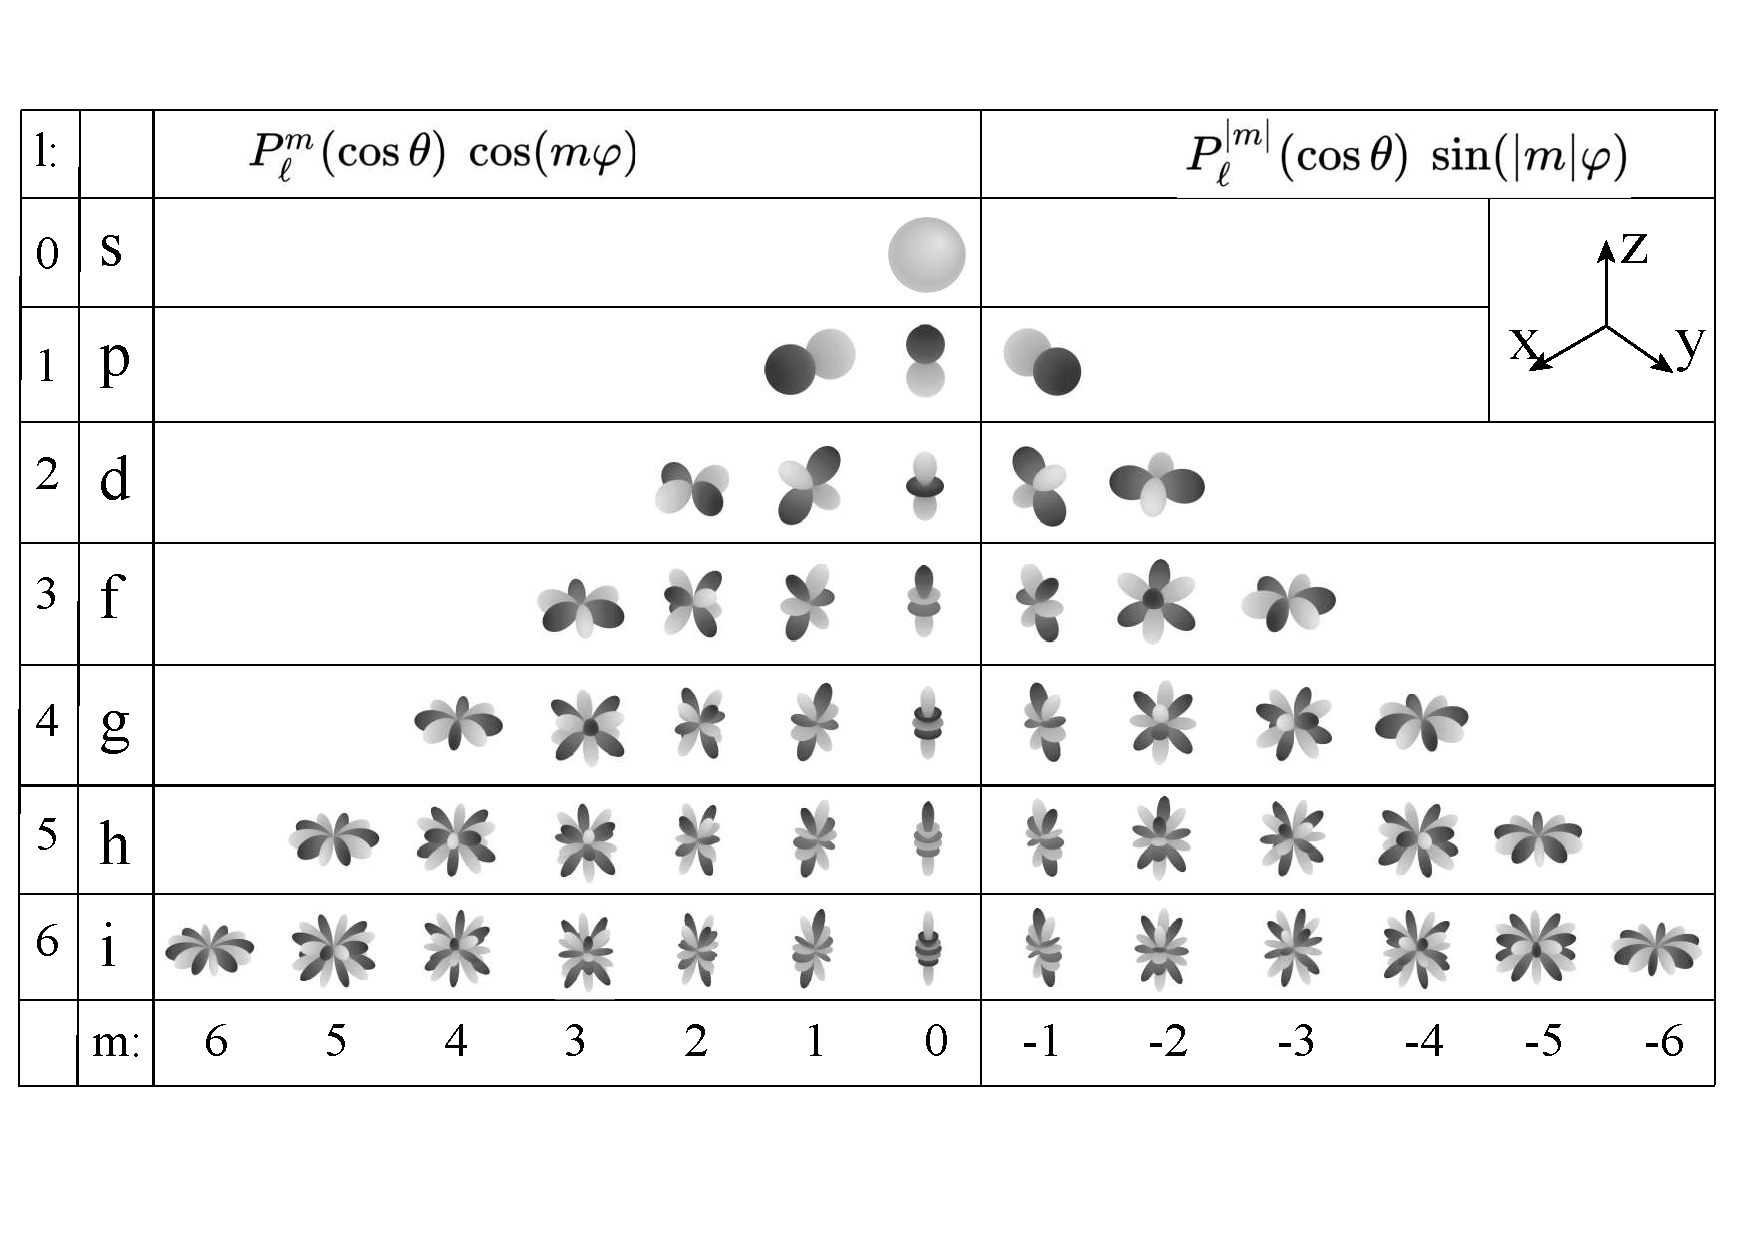
\includegraphics[page=1,width=\textwidth]{pictures/Sphericalfunctions.pdf}
	\caption{Reelle Spherical Harmonics. Der Abstand zum 0-Punkt korrespondiert zum Betrag von $Y_l^m$, die helle Oberfläche zeigt positive Werte von $Y_l^m$, dunkle Oberfläche negative Werte an.}
\end{figure}
